\documentclass{article}

\usepackage{amsmath,graphicx,parskip,mathrsfs,subfigure}
\usepackage{fancyhdr}
\usepackage{amsthm,amssymb}
\usepackage{setspace}
\usepackage{epstopdf}
\usepackage[left=3cm,right=3cm,top=3cm,bottom=3cm]{geometry}

\pagestyle{fancy}
\lhead{Samuel Huberman}
\chead{MSE1022:Preliminary Report}
\rhead{999157923}

\linespread{1}
\begin{document}

\section*{MD Setup}

\begin{figure}[ht]
\centering
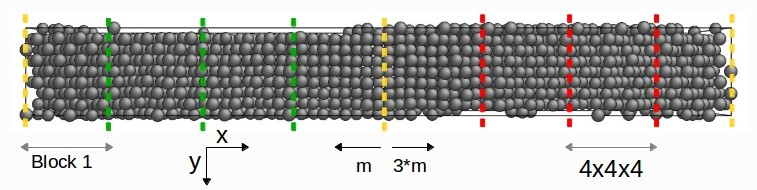
\includegraphics[scale=0.4]{mddom1.jpg}
\caption{MD domain for interface study of fcc Argon at 20K with 2048 atoms}
\label{fig:subfig1}
\end{figure}

\begin{verbatim}
##########MEASURE SED##########################################################
label loop_seed
variable iseed loop 5
variable seed index 11111 22222 33333 44444 55555
clear

#------------READ STRUCTURE-----------------------------------------------------------
units			lj
atom_style		atomic
read_data		interface.data
#group         	        Ar1 type = 1
#group         	        Ar3 type = 3
group			c1 id <= 256
group			c2 id <> 257 512 
group			c3 id <> 513 768
group			c4 id <> 769 1024
group			c5 id <> 1025 1280
group			c6 id <> 1281 1536
group			c7 id <> 1537 1792
group			c8 id >= 1793
#------------LJ Potentials------------------------------------------------------------------
pair_style		lj/cut 2.5
#pair_coeff		1 1 1.0 1.0
pair_coeff		* * 1.0 1.0
pair_modify             shift yes
#------------Variables----------------------------------------------------------------------
#------------LJ Parameters
variable    	kB 		equal 1.3806504e-23 	# [J/K] Boltzmann
variable	sigma_Ar 	equal 3.4e-10 	# m
variable	eps_Ar		equal 1.67e-21	# J
variable	mass_Ar	        equal 6.63e-26	# kg
variable	tau_Ar		equal 2.1423e-12	# s
#------------thermo Parameters
variable    	T_melt 	        equal 300*(${kB}/${eps_Ar})
variable	T_0K		equal 0.001

variable   	dt 		equal 0.002
variable	quench_rate	equal 1.0
variable	quench_length   equal 10000
#------------kappa parameters
variable    	p 		equal 100000 	# correlation length
variable    	s 		equal 10  		# sample interval
variable    	d 		equal $p*$s 		# dump interval 
variable	scaleJ		equal ${eps_Ar}*${sigma_Ar}/${tau_Ar}

#-------------SED parameters
variable	w_step		equal 2^5		#32 steps
variable	w_total	        equal 2^16		#65 some 000 steps
variable	t_total	        equal 2^20		#1048576 steps
variable	num_ffts	equal ${t_total}/${w_total}

#label loop2
#variable b loop 3
#variable T_run index ${T_1} ${T_2} ${T_3}

variable 	T_run 		equal 20*(${kB}/${eps_Ar})
variable	alat		equal 1.5635

#log 	log_quench_$a_$b.lammps
log 	log_heat_${iseed}.lammps

#------------ NVE rescale ---------------------------------------------------------------------	

	velocity 		all create ${T_run} ${seed} rot yes dist gaussian

	fix 			1 all nve
	fix 			2 all temp/rescale 1 ${T_run} ${T_run} 0.01 1.0
	timestep		${dt}
	thermo_style  	custom step temp press etotal vol
	thermo			1000
        dump 2 all cfg 2000 pos.*.cfg id type xs ys zs # Visualize with AtomEye
	run             	500000
#	run             	1000
	unfix 			1
	unfix 			2

#------------ NVE -----------------------------------------------------------------------------	

	fix 			1 all nve
	timestep		${dt}
	thermo_style  	custom step temp press etotal vol
	thermo			1000
	run             	500000	
#	run             	10000
	unfix 			1

#------SED-------------------------------------------------------------------------

label loop_fft
variable ifft loop ${num_ffts}

log 	log_SED_${iseed}_${ifft}.lammps
	reset_timestep  	0
	fix 			1 all nve
	dump 			vel1 c1 custom ${w_step} dump_c1_${iseed}_${ifft}.vel vx vy vz
	dump_modify 		vel1 sort id
	dump 			vel2 c2 custom ${w_step} dump_c2_${iseed}_${ifft}.vel vx vy vz
	dump_modify 		vel2 sort id
	dump 			vel3 c3 custom ${w_step} dump_c3_${iseed}_${ifft}.vel vx vy vz
	dump_modify 		vel3 sort id
	dump 			vel4 c4 custom ${w_step} dump_c4_${iseed}_${ifft}.vel vx vy vz
	dump_modify 		vel4 sort id
	dump 			vel5 c5 custom ${w_step} dump_c5_${iseed}_${ifft}.vel vx vy vz
	dump_modify 		vel5 sort id
	dump 			vel6 c6 custom ${w_step} dump_c6_${iseed}_${ifft}.vel vx vy vz
	dump_modify 		vel6 sort id
	dump 			vel7 c7 custom ${w_step} dump_c7_${iseed}_${ifft}.vel vx vy vz
	dump_modify 		vel7 sort id
	dump 			vel8 c8 custom ${w_step} dump_c8_${iseed}_${ifft}.vel vx vy vz
	dump_modify 		vel8 sort id
	thermo_style 		custom step temp press vol
	thermo			5000
	timestep		${dt}
	run			${w_total}
	unfix			1
	undump			vel1
	undump			vel2
	undump			vel3
	undump			vel4
	undump			vel5
	undump			vel6
	undump			vel7
	undump			vel8

			next ifft
		jump in.LJArint.SED loop_fft
	next seed
	next iseed
jump in.LJArint.SED loop_seed
\end{verbatim}

\section*{Post-processing}

Using the frequencies and eigenvectors obtained from lattice dynamics calculations using GULP, the normal mode coordinates can be determined
\begin{equation}
\dot{Q}(\pmb{\kappa},\nu,t)=\frac{1}{\sqrt{N}}\sum_{jl}\sqrt{m_j}exp(-i\pmb{\kappa}\cdot\pmb{r}(jl))\pmb{e}^*(j,\pmb{\kappa},\nu)\cdot\dot{\pmb{u}}(jl,t)
\end{equation}
where atom $j$ is in unit cell $l$ of a system with a total number of atoms $N$. $\pmb{\kappa},\nu$ correspond to the phonon mode of wavevector $\pmb{\kappa}$ and dispersion branch $\nu$. $\pmb{e}^*(j,\pmb{\kappa},\nu)$ is the complex conjugate of the eigenvectors obtained from GULP. ${\pmb{u}}(jl,t)$ is the velocity of atom $jl$. By taking a series of velocity samples from the MD simulation of time interval (in signal processing terminology, this is known as lag which is symbolically represented here by $t$) an order of magnitude shorter than inverse of the highest frequency present in the system and using Equation 1 to project the sampled velocities onto the eigenvectors, the autocorrelation of the normal modes can calculated by
\begin{equation}
C(\pmb{\kappa},\nu,t)=\lim_{T->\infty}\frac{1}{T}\int_{0}^{T}Q(\pmb{\kappa},\nu,t+t')Q(\pmb{\kappa},\nu,t')dt'
\end{equation}
The spectral energy density (SED), from the Wiener-Khintchine theorem, is thus
\begin{equation}
C(\pmb{\kappa},\nu,\omega)=\int_{-\infty}^{\infty}C(\pmb{\kappa},\nu,t)e^{-i\omega t}dt
\end{equation}
which is a Lorentzian curve centered at $\omega_0(\pmb{\kappa},\nu)$
\begin{equation}
C(\pmb{\kappa},\nu,\omega)=\frac{C_0(\pmb{\kappa},\nu)}{2}\frac{\Gamma(\pmb{\kappa},\nu)/\pi}{(\omega_0(\pmb{\kappa},\nu)-\omega)^2+\Gamma(\pmb{\kappa},\nu)}
\end{equation}
The half width at half maximum of the Lorentzian is related by anharmonic lattice dynamic theory to phonon lifetime by
\begin{equation}
\tau_{p-p}(\pmb{\kappa}, \nu)=\frac{1}{2\Gamma(\pmb{\kappa},\nu)}
\end{equation}
This procedure, from the velocity projection to the Lorentzian curve fitting, was automated using MATLAB.

\section*{Sample results}
Using the output from the above LAMMPS script for the interface (a more basic one is used for the bulk case), the post-processing, performed on block 1, produced the following sample SED plots:

\begin{figure}[ht]
\centering
\subfigure[\small{$\pmb{\kappa}=[0,1,0]$},$\nu=$TA]{
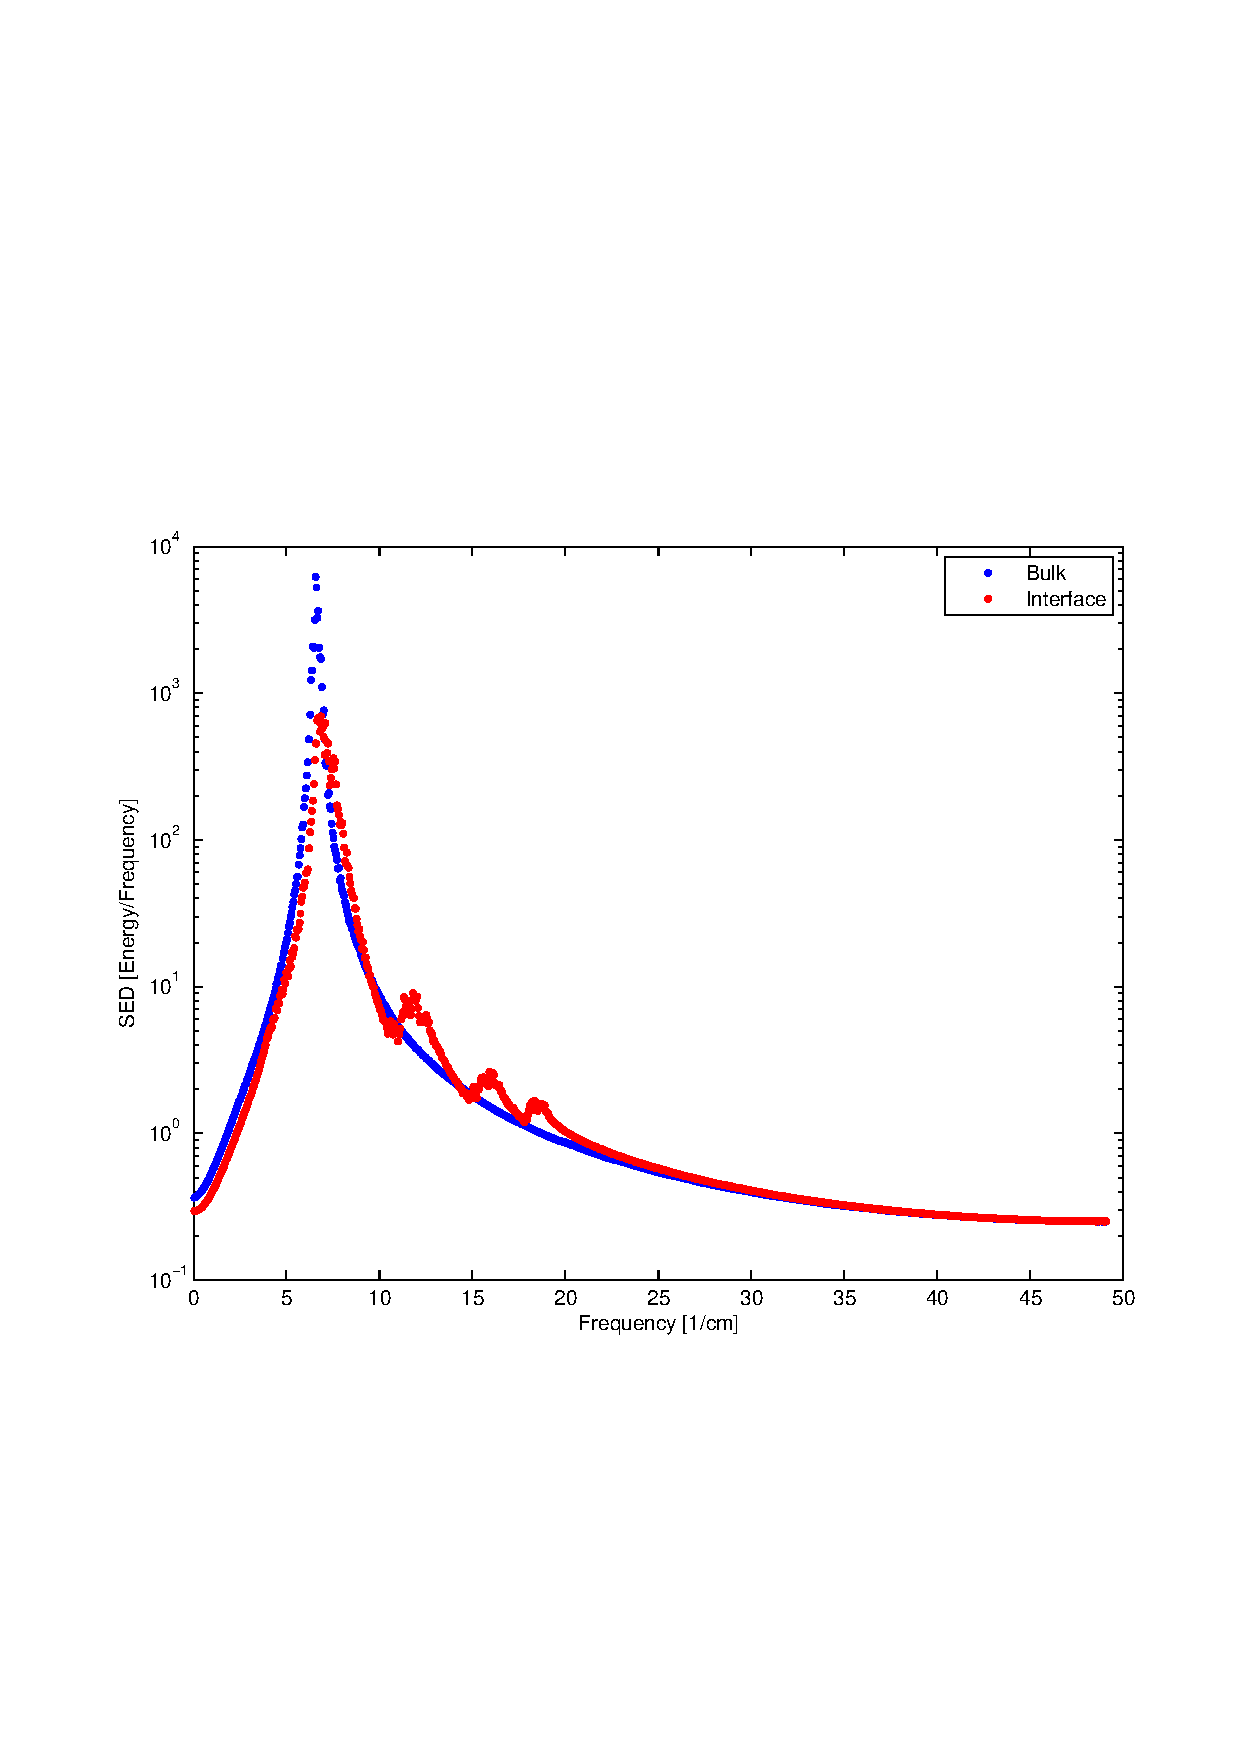
\includegraphics[scale=0.35]{peak_010}
}
\subfigure[\small{$\pmb{\kappa}=[1,0,0]$,$\nu=$TA}]{
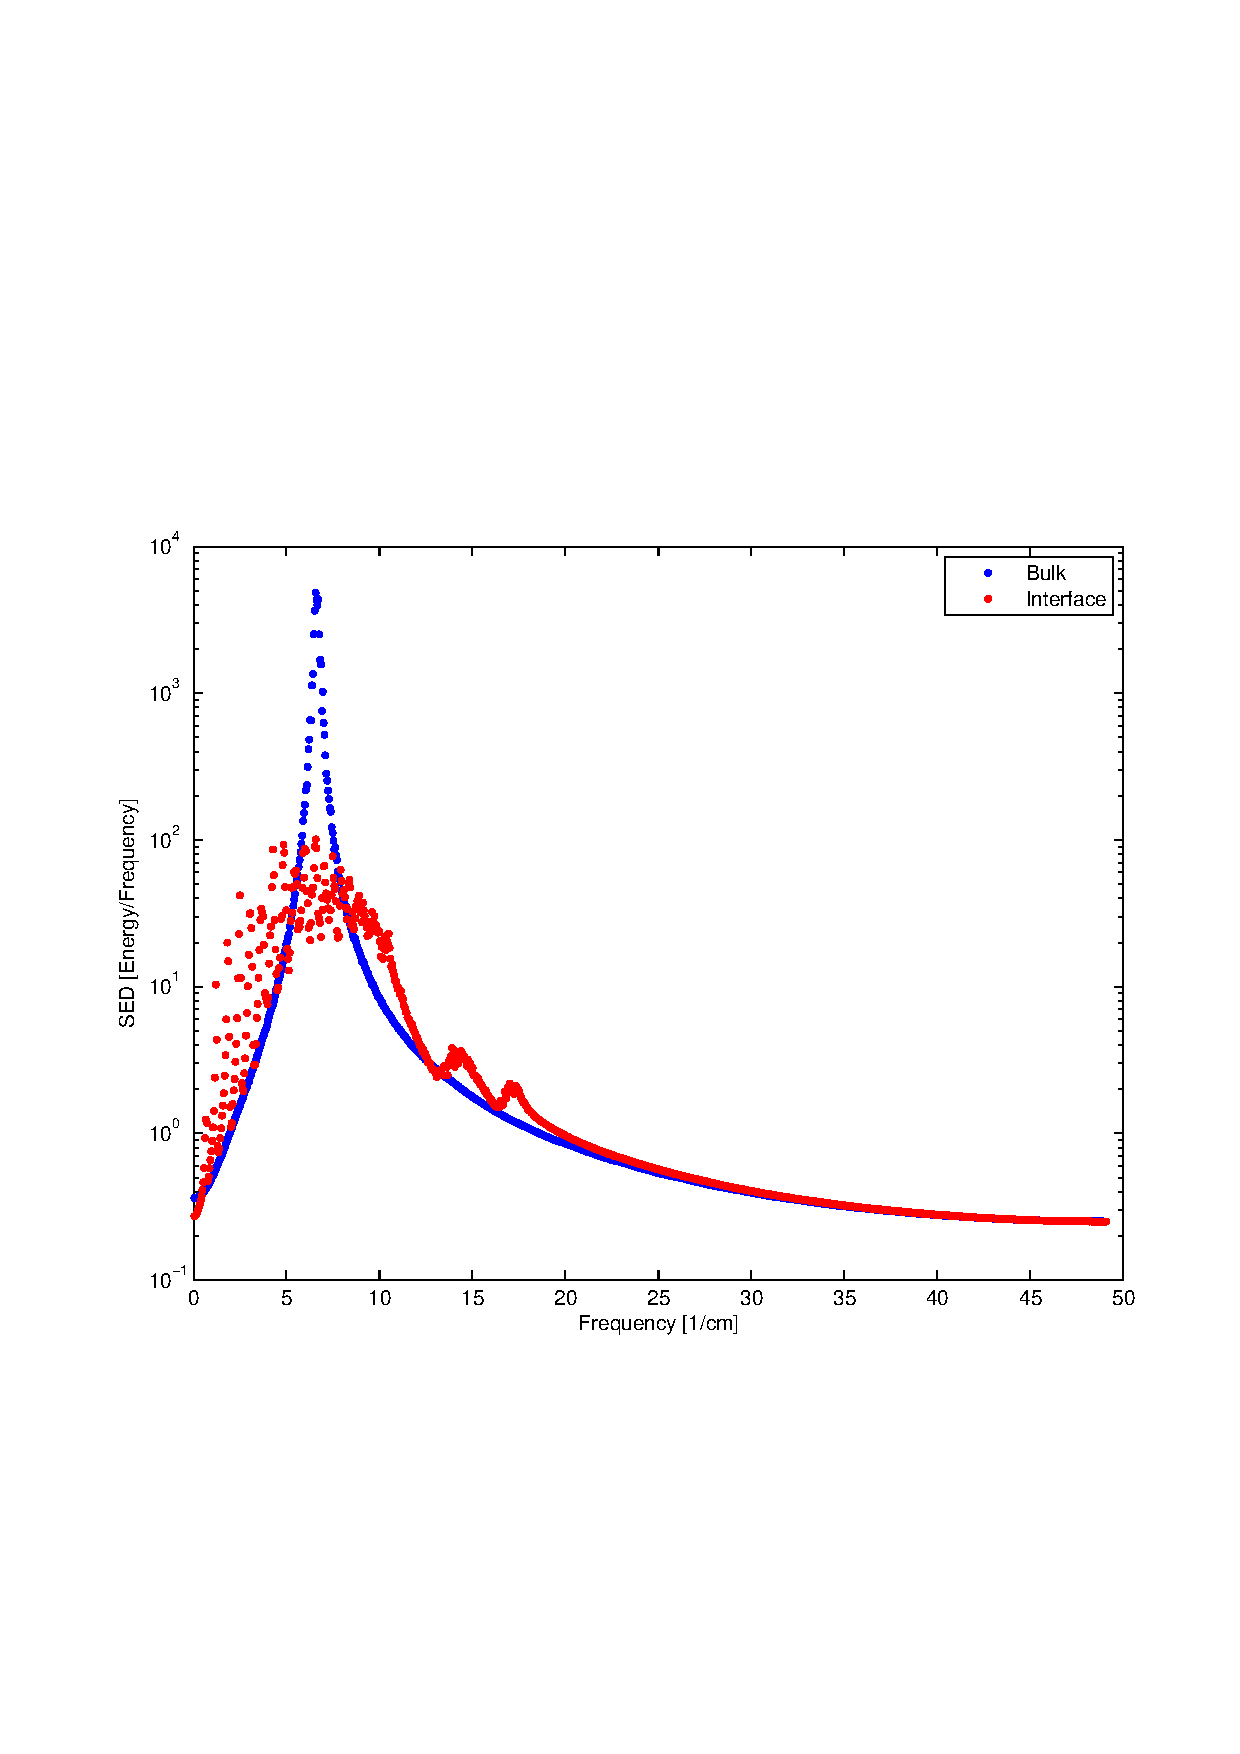
\includegraphics[scale=0.35]{peak_100}
}
\end{figure} 
\section*{Future Steps}
The challenge, at this point, is to explain the trend observed in these figures from a fundamental perspective. What is causing the secondary bumps in these curves? For certain phonon modes, why does the presence of the interface destroy the Lorentzian form? Perhaps changing the number of blocks (changing the periodicity of the superlattice) from the interface will provide insight into these questions.

\end{document}

